\documentclass[tikz,border=4pt]{standalone}
\begin{document}
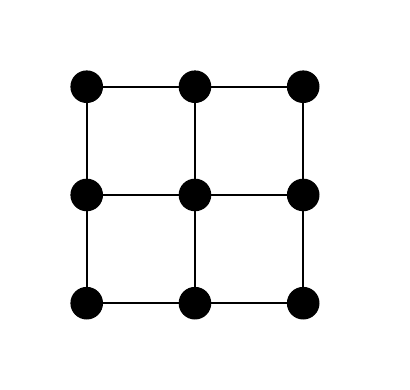
\begin{tikzpicture}[x=.025cm,y=-.025cm]
\path[use as bounding box] (0,0) rectangle (180,170);
\path[draw=black,fill=none,line width=0.7150000000000001pt] (30,30) -- (140,30);
\path[draw=black,fill=none,line width=0.7150000000000001pt] (30,30) -- (30,140);
\path[draw=black,fill=none,line width=0.7150000000000001pt] (30,85) -- (140,85);
\path[draw=black,fill=none,line width=0.7150000000000001pt] (85,30) -- (85,140);
\path[draw=black,fill=none,line width=0.7150000000000001pt] (30,140) -- (140,140);
\path[draw=black,fill=none,line width=0.7150000000000001pt] (140,30) -- (140,140);
\path[draw=black,fill=black] (30,30) circle[radius=0.2cm];
\path[draw=black,fill=black] (30,85) circle[radius=0.2cm];
\path[draw=black,fill=black] (30,140) circle[radius=0.2cm];
\path[draw=black,fill=black] (85,30) circle[radius=0.2cm];
\path[draw=black,fill=black] (85,85) circle[radius=0.2cm];
\path[draw=black,fill=black] (85,140) circle[radius=0.2cm];
\path[draw=black,fill=black] (140,30) circle[radius=0.2cm];
\path[draw=black,fill=black] (140,85) circle[radius=0.2cm];
\path[draw=black,fill=black] (140,140) circle[radius=0.2cm];
\end{tikzpicture}
\end{document}
